今回使っているのはラズパイで制御する4輪走行ロボットである(Fig.\ref{robot_img}),
人間や昆虫の走行特徴に近似するため,その場で曲がり,方向転換が可能である.
ロボットの頭にカメラ(D)をつけていて,入力データを収集する.
E,Fは左右のモーター,独自で左右の車輪を制御して,ロボットを動かす.
A,B,Cは右,中央,左の距離センサ,先行研究で使っていたが,本文は使っていない.
ロボット幅は13.5cm.長さは20.2cm.高さは12.2cmである.

\vspace{-4mm}
\begin{figure}[htb]
    \centering
    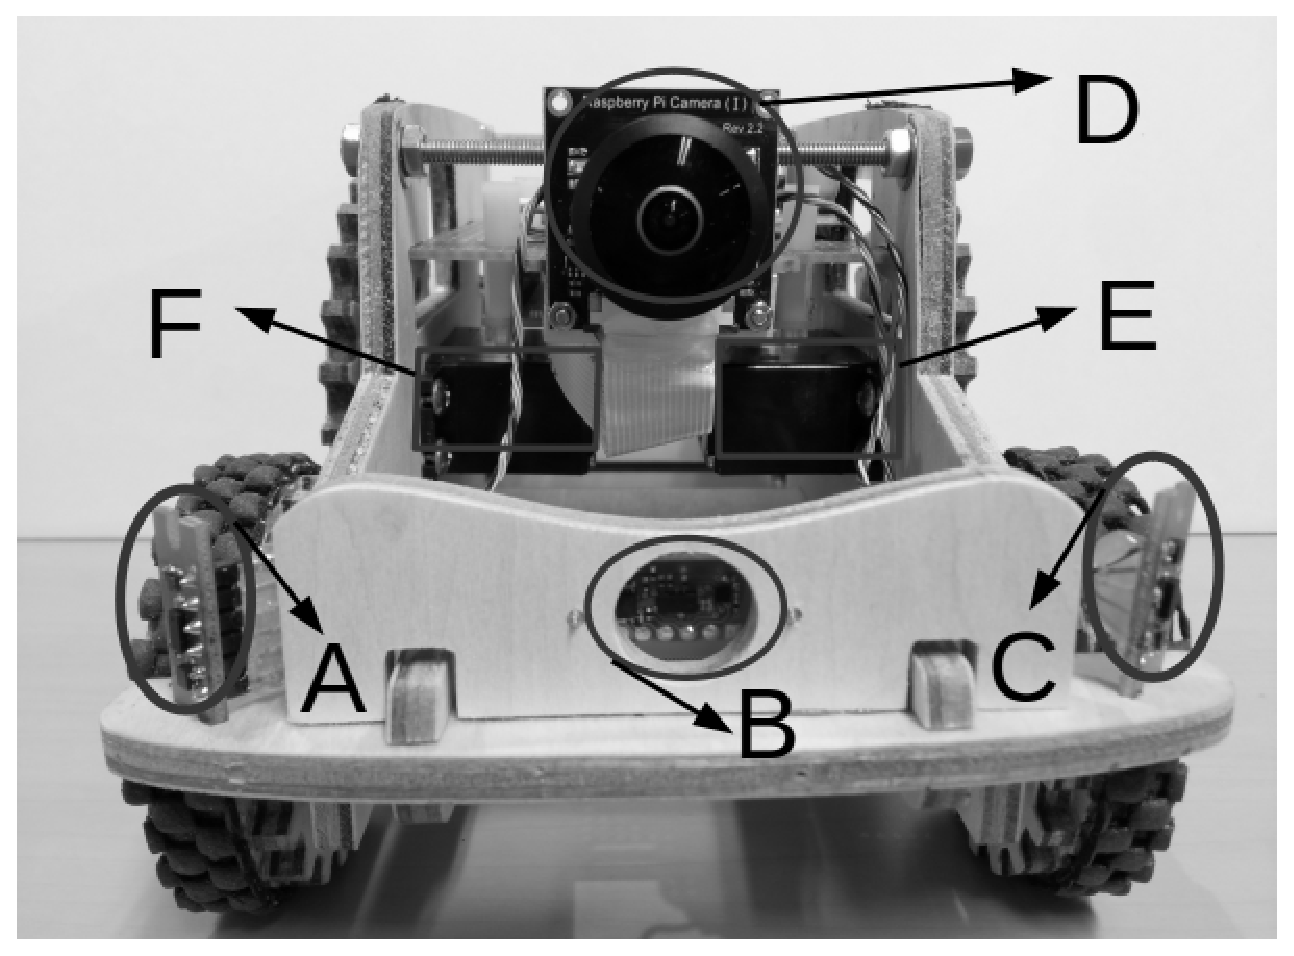
\includegraphics[width=0.4\linewidth]{robot1.eps}
  \label{robot_img}
    \caption{ロボット正面図}
\end{figure}




